\documentclass[10pt,twoside]{fernandes_supp} 
%Default opts:9pt,twocolumn,twoside
\graphicspath{{images_supp/}}

\newcommand{\KB}[1]{\noindent\color{blue}$\Longrightarrow$ #1\normalcolor}
\newcommand{\mf}[1]{\colorbox{blue!10}{\color{color3}#1}}

\title{Supplemental Information:\\ Harnessing  Design Principles from Glass Sponges for Structurally Robust Lattice Structures}

\author[1]{Matheus C. Fernandes}
\author[2]{James C. Weaver}
\author[1,3,*]{Katia Bertoldi}

\affil[1]{John A. Paulson School of Engineering and Applied Sciences -- Harvard University, Cambridge, MA 02138}
\affil[2]{Wyss Institute -- Harvard University, Cambridge, MA 02138}
\affil[3]{Kavli Institute -- Harvard University, Cambridge, MA 02138}
\affil[*]{Corresponding author: \href{mailto:bertoldi@seas.harvard.edu}{bertoldi@seas.harvard.edu}}

\begin{document}
\maketitle
% \doublespace
% \linenumbers
\section{Structure of the Hexactinellid sponge \textit{Euplectella aspergillum}}\label{sec:params}
The periodic structures investigated in this study are inspired by the skeleton of the Hexactinellid sponge \textit{Euplectella aspergillum (sp.)}, commonly known as the "Venus' flower basket". In this section we provide a detailed description of the sponge geometry and measured dimensions.

\Cref{Sponge} shows a photograph of the entire skeleton of the \textit{Euplectella sp.}, and its intricate, cylindrical cage-like structure (20 to 25cm long, 2 to 4 cm in diameter) \citep{aizenberg2005}. The surface of the cylinder consists of a regular square lattice composed of a series of cemented vertical and horizontal struts with circular cross-section. The cell spacing between horizontal and vertical struts was reported  to be $L\approx 2.5$mm \citep{weaver2007}, while their diameter was measured to be $D_{nd}\approx 0.25$mm \citep{weaver2007}. Besides the horizontal and vertical struts, there is an additional set of diagonal elements, intersecting in a manner that creates a series of alternating open and closed cells, reminiscent of a checkerboard pattern \citep{weaver2007}. Although these diagonal elements are not as ordered as the horizontal and vertical ones, it has been shown that they can be approximated with two diagonal struts that are offset from the nodes  (vertex joints between non-diagonal elements) and form octagonal openings (\cref{Sponge}(d)). To estimate the volume ratio between diagonal and non-diagonal elements, we took high resolution photographs of the sponge and performed image segmentation to segregate the projected area of the vertical/horizontal and diagonal spicules. Using this approach, the projected area ratio of non-diagonal to diagonal elements was found to be $A_{nd}/A_{d}\approx1.4$. Note that here, and in the following, the subscripts $d$ and $nd$ are used to indicate diagonal and non-diagonal (i.e. horizontal and vertical) elements, respectively. 

Finally, it should also be noted that the sponge is reinforced by external ridges that extend perpendicular to the surface of the cylinder and spiral the cage at an angle of $45^\text{o}$. However, in this paper we do not report the effects of these ridges on it's structural performance.

\begin{figure}[H]
    \centering
    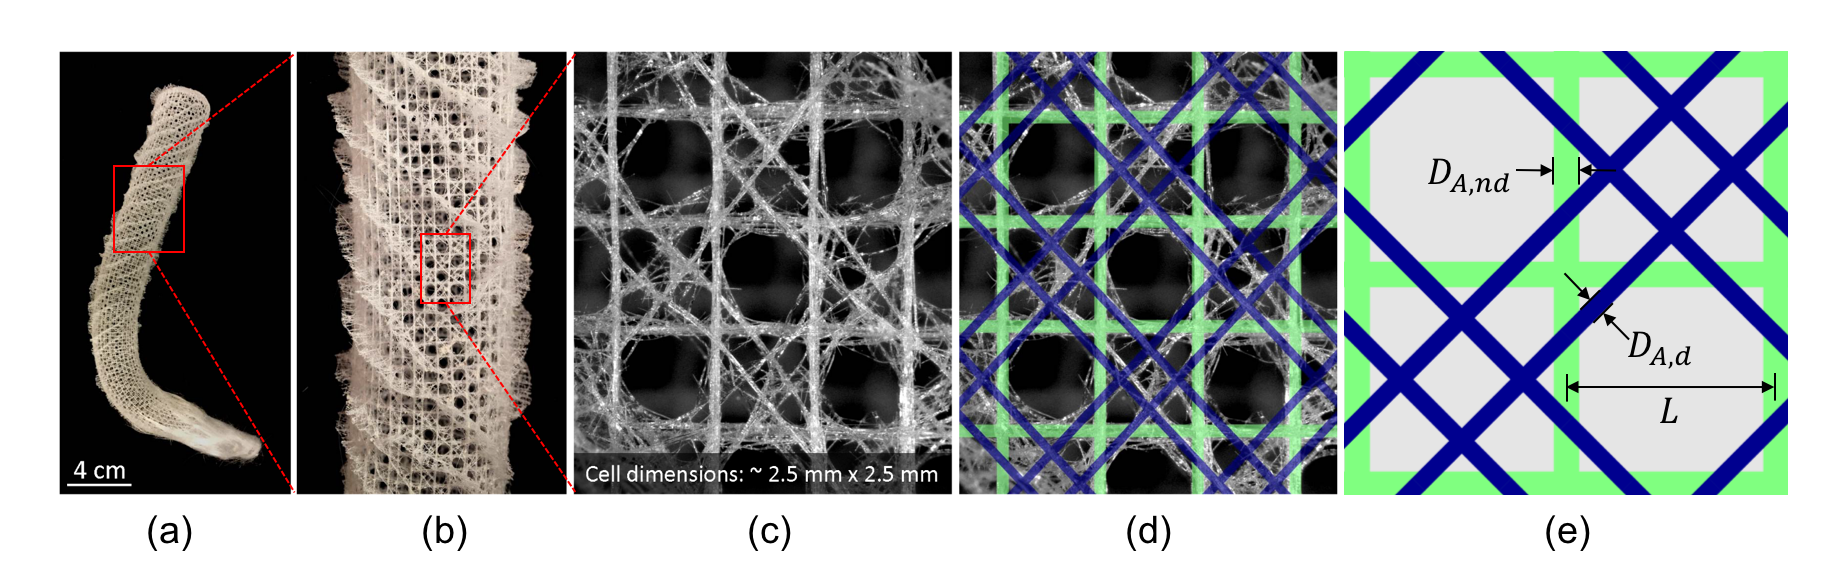
\includegraphics[width=0.9\linewidth]{SFig1.png}
    \caption{\textbf{Hexactinellid sponge \textit{Euplectella aspergillum.}} (a)-(b) Full-frame photo of sponge.  (c)  Close up microscope image of the sponge. (d) Comparison between the idealized model (green and blue lines) and the sponge structure. (e) Unit cell of the idealized model.}
    \label{Sponge}
\end{figure}

\section{Designs Considered}
In this study, we focus on four different lattice configurations constrained to deform in an in-plane setting only. In an effort to provide a fair performance compassion between the different designs all of the respective lattice configurations, the total amount of material (i.e. volume or mass) is conserved. Moreover,  we consider a fixed volume ratio between non-diagonal and diagonal elements (chosen to match the sponge geometry) and two different shapes for the cross section of all lattice members: circular and rectangular.  For circular cross-sections  we stay consistent with the geometry found within the biological species. However, since slender members with circular cross section easily buckle out-of-plane when the structure is subjected to compression we must mitigate the issue by pursuing a plane-strain structure such that it's depth slenderness ratio is sufficiently deep to avoid out-of-plane buckling. In order to address this, we converted the biological observations of the cylindrical cross-section into a polygonal section. For this new cross-section type, we assume the structure to be sufficiently deep in plane in comparison the structural length scale (plane strain assumption) to avoid out of plane deformation. The out-of-plane slenderness is scaled accordingly with mass to maintain the depth across all elements constant. A parametric simulation on depth was analyzed to determine the minimum cross-section depth required to prevent out-of-plane buckling. Once the overall minimum depth for all geometries was chosen a factor of safety of 1.5 was added for the finial depth. The approach for minimum out-of-plane depth was further verified experimentally and the value was determined sufficient.

For this new cross-section type, we assume the structure to be sufficiently deep in plane in comparison the structural length scale (plane strain assumption) to avoid out of plane behavior. The cross-section is scaled accordingly with mass while maintaining the depth across all elements constant. In the subsequent sections, we describe in detail the unit cells for the four different designs (Designs A-D).

\subsection{Design A}
Design A is inspired by the sponge structure and consists of a square grid  reinforced by a double diagonal system (see \cref{DesignA}). 
\subsubsection{Circular cross section} 
If we assume that the horizontal and vertical struts have length $L$ and circular cross section  with diameters $D_{A,nd}$, their volume and projected-area in the unit cell are given by 
\begin{equation}\label{V1}
V_{A,nd}=8 L \left(\pi\frac{D^2_{A,nd}}{4}\right)=2 L \pi D^2_{A,nd}
\end{equation}
and
\begin{equation}\label{A1}
A_{A,nd}=8 L D_{A,nd},
\end{equation}
respectively. Note that in this study we use 
\begin{equation}
\frac{D_{A,nd}}{L}=0.1,
\end{equation}
since this is the aspect ratio measured for the sponges (see \cref{sec:params}).

Moreover, as for the case of the sponge, the diagonal elements are assumed to form an octagonal opening on every other cell. As such, the diagonals intersect the horizontal and vertical struts at a distance $\Delta L=L/(\sqrt{2}+2)$ from the nodes and their  volume and projected area in the unit cell are
\begin{equation}\label{V2}
V_{A,d}=8 \sqrt{2} L\left(\pi\frac{D^2_{A,d}}{4}\right)=2\sqrt{2}L \pi D^2_{A,d},
\end{equation}
and
\begin{equation}\label{A2}
A_{A,d}=8\sqrt{2} L D_{A,d},
\end{equation}
respectively. Since the projected area ratio of the non-diagonal to diagonal elements in the sponge has been measured to be 
\begin{equation}
\frac{A_{A,nd}}{A_{A,d}}=1.4,
\end{equation}
by substituting \cref{A1} and \cref{A2} into the equation above we find that for Design A
\begin{equation} \label{DA}
D_{A,nd}=1.4\sqrt{2}D_{A,d}\approx 2 D_{A,d}.
\end{equation}
Substitution of \cref{DA} into \cref{V1} and \cref{V2} yields 
\begin{equation}
\frac{V_{A,nd}}{V_{A,d}}=\frac{2 L \pi D^2_{A,nd}}{2\sqrt{2}L \pi D^2_{A,d}}=2\sqrt{2}
\end{equation}
and
\begin{equation}\label{VT}
V_{A,T}=V_{A,nd}+V_{A,d}=2\pi L (D_{A,nd}^2+\sqrt{2} D_{A,d}^2)=2\pi L D_{A,nd}^2 \left(1+\frac{1}{2\sqrt{2}}\right),
\end{equation}
where $V_{A,T}$ indicates the total volume of the unit cell for Design A. 

Finally, it is important to note that in this study we use Design A as our base model, and thus constrain the total volume of all the other unit cell designs to be equal to that of Design A, namely,
\begin{equation}\label{con1}
V_{\alpha,d}+V_{\alpha,nd}={V}_{A,T}=2\pi L D_{A,nd}^2 \left(1+\frac{1}{2\sqrt{2}}\right),
\end{equation}
with $\alpha=$ B, C and D.
Finally,  for Designs B and C, which comprise diagonal elements, we also  constrain the volume ratio of the non-diagonal to diagonal elements to be the same as in Design A
\begin{equation}\label{con2}
\frac{V_{\alpha,nd}}{V_{\alpha,d}}=\frac{V_{A,nd}}{V_{A,d}}=2\sqrt{2},
\end{equation}
with $\alpha=$ B and C.

\begin{figure}[H]
    \centering
    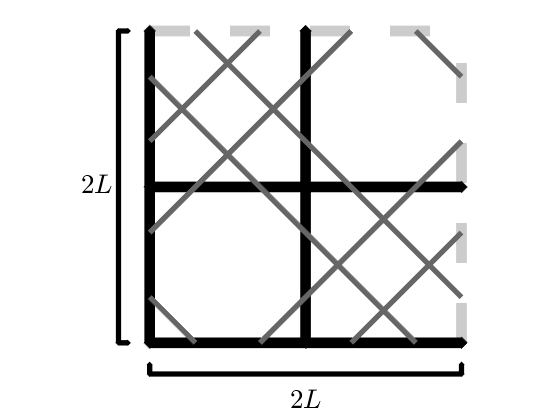
\includegraphics[width=0.45\linewidth]{SFig2.png}
    \caption{{\bf Unit cell for Design A.} This design is inspired by the sponge structure and consists of a square grid  reinforced by a double diagonal system. The horizontal and vertical struts have length $L$ and circular cross section with diameter $D_{A,nd}$ and, as with the sponge, we assume $D_{A,nd}/L=0.1$. The diagonal elements have a circular cross section  with diameter $D_{A,d}=2 D_{A,nd}$.}
    \label{DesignA}
\end{figure}

\subsubsection{Rectangular cross-section}
From $A_{nd}/A_d\approx 1.4$ we know that the volume is the same given that the in-plane dimension is constant, namely $V_{nd}/V_d\approx 1.4$ . Assuming that the in-plane thickness is given by $t$, we can derive the following volumes for the diagonal and non-diagonal, respectively:
\begin{equation}
	V_{A,nd}=8LD_{A,nd}t
\end{equation}
\begin{equation}
	V_{A,d}=8\sqrt{2}LD_{A,d}t
\end{equation}
Let us enter this into our biological observation, which yields:
\begin{equation}
	\frac{V_{A,nd}}{V_{A,d}}\approx 1.4\approx\sqrt{2}=\frac{8LD_{A,nd}t}{8\sqrt{2}LD_{A,d}t}
\end{equation}
Therefore, we can simplify this relationship as
\begin{equation}
	D_{A,nd}=2D_{A,d}
\end{equation}

\subsection{Design B}
Design B is similar to the sponge design (Design A) and is likewise characterized by an alternation of open and closed cells (\cref{DesignB}). However, instead of having two diagonals offset from the nodes, here we only have one diagonal passing through the nodes and crossing every other cell. 
\subsubsection{Circular cross section}
It follows that the non-diagonal and diagonal volumes are given by
\begin{equation}
V_{B,nd}=V_{A,nd}=2\pi L D_{B,nd}^2
\end{equation}
and
\begin{equation}
V_{B,d}=2\sqrt{8} L \left(\pi \frac{{D}_{B,d}^2}{4}\right),
\end{equation}
respectively.
Using the constraints provided by \cref{con1} and \cref{con2}, as well as the above volumes, we  obtain 
\begin{equation}
{{D}_{B,nd}}={{D}_{A,nd}}
\end{equation}
and
\begin{equation}
\frac{{D}_{B,d}}{{D}_{B,nd}}=\frac{1}{\sqrt{2}}.
\end{equation}

\begin{figure}[H]
    \centering
    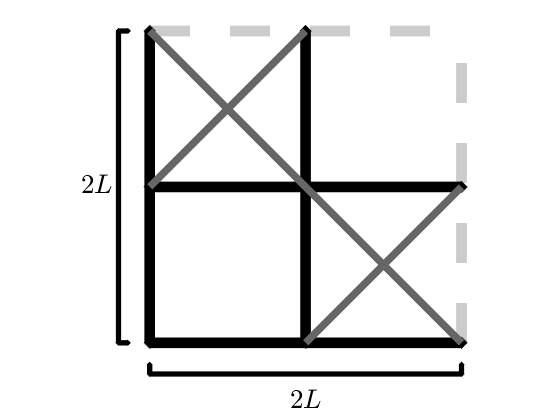
\includegraphics[width=0.45\linewidth]{SFig3.png}
    \caption{{\bf Unit cell for Design B.} This design is still characterized by an alternation of open and closed cells. However, instead of having two  diagonals offset from the nodes, here we only have one diagonal passing through the nodes and crossing every other cell. The horizontal and vertical struts have length $L$ and a circular cross section with diameter $D_{B,nd}$. The diagonal elements have a circular cross section  with diameter $D_{B,d}={D_{B,nd}}/{\sqrt{2}}$.}
    \label{DesignB}
\end{figure}

\subsubsection{Rectangular cross section}

For this design the volume of non-diagonal elements remain the same, namely,
\begin{equation}
		V_{B,nd}=8LD_{B,nd}t.
\end{equation}
However, the volume for the diagonal elements will is different as a result the change in total length, namely,
\begin{equation}
		V_{B,d}=4\sqrt{2}LD_{A,d}t.
\end{equation}
In in effort to maintain a constant volume ration between the diagonally reinforced designs, we use the same volume ratio as per observation
\begin{equation}
		\frac{V_{B,nd}}{V_{B,d}}\approx 1.4\approx\sqrt{2}=\frac{8LD_{B,nd}t}{4\sqrt{2}LD_{B,d}t}
\end{equation}
which simplifies to
\begin{equation}
	D_{B,nd}=D_{B,d}
\end{equation}
and
\begin{equation}
	D_{B,nd}=D_{A,nd}
\end{equation}

\subsection{Design C}
Design C is inspired by the town lattice truss design introduced by architect Ithiel Town in 1820 \citep{waddell1916} and consists of every cell being reinforced by diagonal trusses passing through the nodes (see \cref{DesignC}).

\subsubsection{Circular cross section}
For this design, the non-diagonal and diagonal volumes of the unit cell are given by:
\begin{equation}
V_{C,nd}=V_{A,nd}=2 L \pi D^2_{A,nd}
\end{equation}
and
\begin{equation}
V_{C,d}=V_{A,d}=2\sqrt{2}L \pi D^2_{A,d},
\end{equation}
respectively.
Using the constraints provided by \cref{con1} and \cref{con2} we  obtain 
\begin{equation}
{{D}_{C,nd}}={{D}_{A,nd}}
\end{equation}
and
\begin{equation}
\frac{{D}_{C,d}}{{D}_{C,nd}}=\frac{1}{2}.
\end{equation}

\begin{figure}[H]
    \centering
    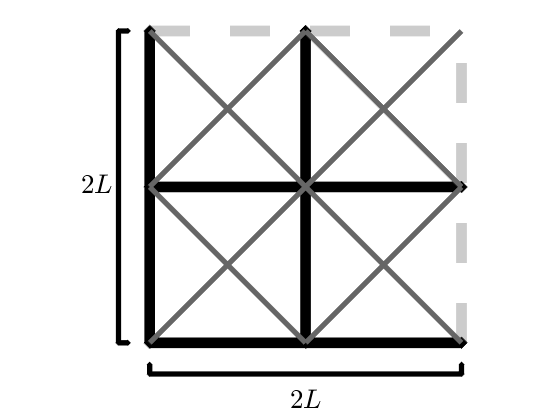
\includegraphics[width=0.45\linewidth]{SFig4.png}
    \caption{{\bf Unit cell for Design C.} This design consists of a square grid with all cells being reinforced by diagonal trusses passing through the nodes.  The horizontal and vertical struts have length $L$ and a circular cross section with diameter $D_{C,nd}$. The diagonal elements have a circular cross section  with diameter $D_{C,d}={D_{C,nd}}/{2}$.}
    \label{DesignC}
\end{figure}

\subsubsection{Rectangular cross section}
Because the total length of the diagonal and non-diagonal elements are the same as for Design A, we obtain the same diameters for the elements, namely,
\begin{equation}
D_{A,nd}=2D_{A,d}
\end{equation}
and
\begin{equation}
D_{C,nd}=D_{A,nd}
\end{equation}


\subsection{Design D} 
Design D comprises only the square grid without diagonal reinforcement (\cref{DesignD}) and is well known to be unstable and very limited in resisting shear forces \citep{gibson1999,deshpande2001}. As such, for this design we allocate the total material volume to the non-diagonal elements.

\subsubsection{Circular cross section}
Since
\begin{equation}
V_{D,T}=V_{D,nd}=V_{A,nd}=2\pi L D_{D,nd}^2,
\end{equation}
using the constraint provided by \cref{con1} we obtain
\begin{equation}
{D_{D,nd}}={D_{A,nd}}\sqrt{1+\frac{\sqrt{2}}{4}}. 
\end{equation}

\begin{figure}[H]
    \centering
    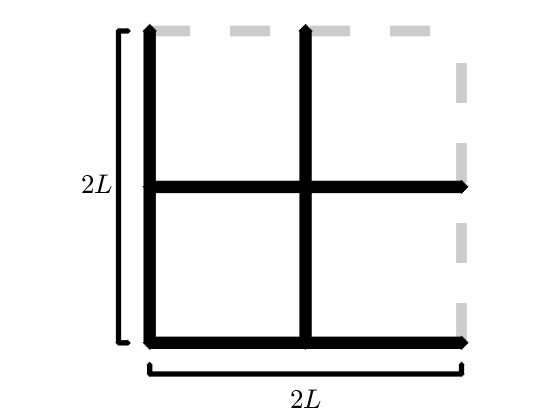
\includegraphics[width=0.45\linewidth]{SFig5.png}
    \caption{{\bf Unit cell for Design D.} This design consists of a square grid without diagonal reinforcement.  The horizontal and vertical struts have length $L$ and a circular cross section with diameter $D_{D,nd}$.}
    \label{DesignD}
\end{figure}

\subsubsection{Rectangular cross-section}
For this design, because it does not contain any diagonal elements, we must allocate the total volume of the structure fully on the non-diagonal elements. Thus we can formulate the total volume of Design A as
\begin{equation}
	V_{A,nd}+V_{A,d}=(D_{A,nd}+\sqrt{2}D_{A,d})8Lt
\end{equation}
Using the relationship between the non-diagonal thickness and diagonal thickness, we obtain
\begin{equation}
V_{A,nd}+V_{A,d}=\left(1+\frac{1}{\sqrt{2}}\right)8LtD_{A,nd}
\end{equation}

We can build a relationship between Design A and Design D through the total volume, such that the total volume of Design A is the same as the total volume of Design D
\begin{equation}
\left(1+\frac{1}{\sqrt{2}}\right)8LtD_{A,nd}=8LtD_{D,nd}
\end{equation}
which yields a relationship between the thicknesses of the non diagonal elements as
\begin{equation}
	D_{D,nd}=\left(1+\frac{1}{\sqrt{2}}\right)D_{A,nd}
\end{equation}

\section{Optimization Analysis}
For the optimization portion of the work presented in the main article we used a stochastic, derivative-free evolutionary method called Covariance Matrix Adaptation Evolution Strategy (CMA-ES) implementation in Python \citep{hansen2003}. The algorithm parameters (continuous input variables) are: the structure's mass ratio $\lambda$ (keeping the total structure volume constant, as well as distributing the mass evenly through all diagonal and non-diagonal elements respectively) and the separation of the even numbered diagonal elements from the non-diagonal junction. Separate instances of the optimization algorithm are analyzed for different numbers of diagonal reinforcements. For simulations with odd number of diagonal re-enforcements, only an even number of diagonals are separated while keeping one diagonal going through the non-diagonal junction in order to ensure geometry symmetry. The algorithm's initial values are chosen to be in the center of the design space, namely, $\lambda=1$ and diagonal separation$=0.5*L$. The optimization is run under a uniaxial loading condition in the direction parallel non-diagonal elements. In order to maintain reasonable computational complexity, the optimization was run on the unit cell constructed using one dimensional beams with node seeding of at least 1/20 of each beam length. The covariance matrix is initialized uniformly with standard deviation \mf{ADD HERE}.

In optimization results presented in the main article, we seek to maximize the singly objective target function for the critical buckling load. However, an equivalent analysis is performed to maximize the critical buckling strain as the target response. This analysis is presented in \cref{BucklingOptimization}. Similarly, the same analysis was performed on the elastic stiffness of the structure and yields a trivial result leading to maximizing the allocation of mass to the non-diagonal elements through the mass ratio.

\begin{figure}[H]
    \centering
    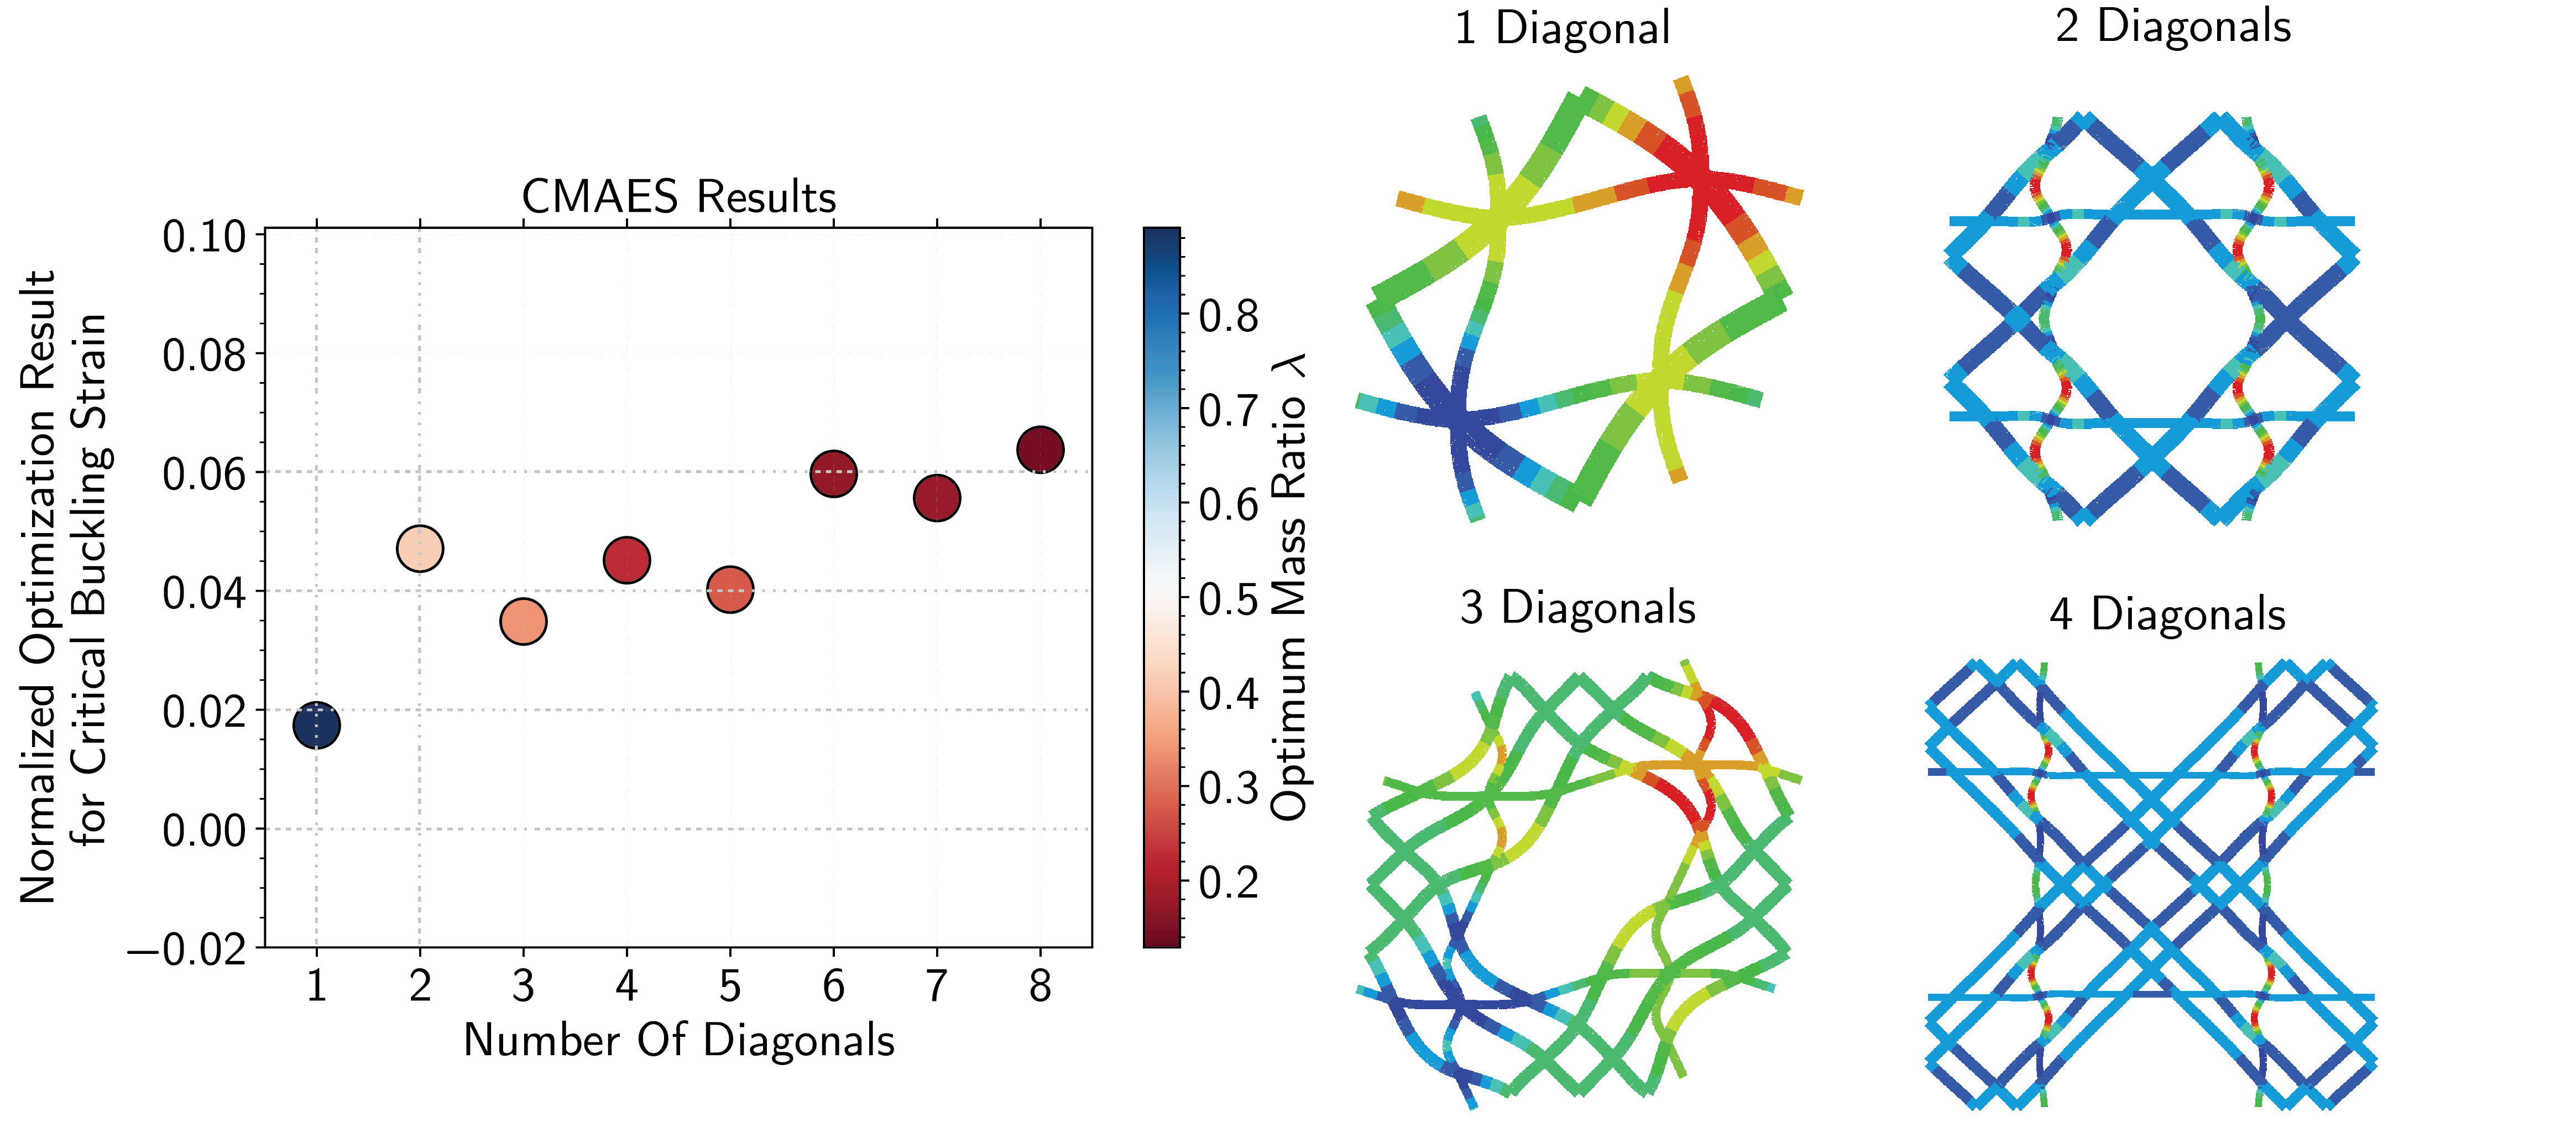
\includegraphics[width=0.9\linewidth]{SFig6.png}
    \caption{{\bf Buckling Optimization.} Graph shows optimal value of critical buckling strain for varying number of diagonals. For all simulations, the total mass of the structure is maintained constant while the mass-ratio is allowed to vary. Furthermore, the diagonal separation for each pair of diagonal is allowed to vary together ensuring half symmetry of the structure at all times. The optimization is run under a uniaxial loading condition. The color of each point on the graph corresponds to the optimum value of mass ratio for that particular number of diagonals. Four deformation plots of the optimum structure and buckling modes are provided on the right for their respective number of diagonals.}
    \label{BucklingOptimization}
\end{figure}

\section{Parameter Exploration}
Include the graphs showing critical buckling strain as a function of parameters.\\
\mf{Add figures for the diagonal}\\
\mf{Add figure for $\lambda$ exploration}\\
\mf{Make sure to include this analysis for both, rectangular cross-section and circular cross-section}\\
\mf{Write this section}
\subsection{Cylindrical Cross Section}
\subsection{Rectangular Cross Section}

\section{Additional numerical results}
\mf{Write this section}

 In this section we validate the RVE domain size by checking the response of larger domain sizes on the critical buckling value. This ensures that there does not exist another critical buckling mode that is limited by our choice of RVE.

\mf{Write about minimum RVE -- how do I convey this message? Should I produce a plot or just verbally state this check?}

\section{Analytical Derivation Of Uniaxial Stiffness}
\mf{Write this section}
%\subsection{Analytical Derivation of Critical Buckling Strain}


% Bibliography
\nocite{aizenberg2005}
\nocite{deshpande2001}
\nocite{miserez2008}
\nocite{weaver2010}

\bibliography{refs}
\bibliographystyle{apalike}
% \bibliographystyle{plainnat}

\end{document}